\documentclass{beamer}

\usepackage[ngerman,english]{babel}
\usepackage[utf8]{inputenc}
\usetheme{Montpellier}
\usepackage{tikz}

\definecolor{beamer@blendedblue}{rgb}{0.3,0.5,0.6}

\setbeamercolor{normal text}{fg=black, bg=white}
\setbeamercolor{alerted text}{fg=red}
\setbeamercolor{example text}{fg=green!50!blue}

\title{Virtual Reality for Sensor Data Analysis}
\subtitle{SW-Projekt SS 2017 Gruppe 5.1}
\author{Gero Birkhölzer \and Johannes Blank \and Alexej Gluschkow \\ \and Fabian Klopfer \and Lisa-Maria Mayer}
\date{Endpräsentation am 25. Juli 2017}



\addtobeamertemplate{frametitle}{}{%
\begin{tikzpicture}[remember picture,overlay]
\node[anchor=north east,yshift=2pt] at (current page.north east) {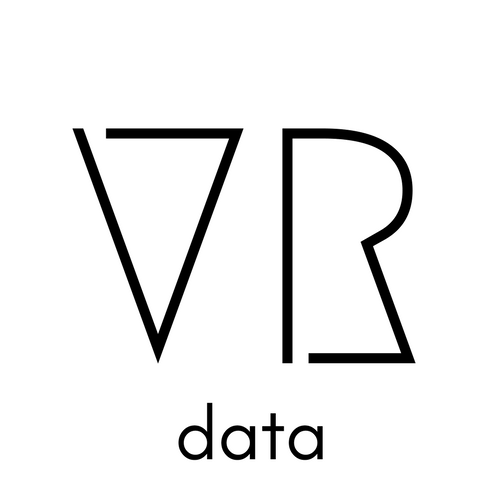
\includegraphics[height=0.8cm]{logo.png}};
\end{tikzpicture}}


\begin{document}


\frame{\titlepage}



\begin{frame}
  \frametitle{Inhalt}
  \tableofcontents%[hideallsubsections]
\end{frame}


\section{Einleitung}

\subsection{Use Case}

\begin{frame}
\frametitle{Use Case}
\begin{itemize}
	\item  Fachbereich Sport will Sporthalle sanieren lassen
	\item Brauchen "Beweise", dass Sanierung notwendig ist
	\item U.a: Lüftungsanlage sanierungsbedürftig
	\item Temperaturdaten aufnehmen und den Verantwortlichen in anschaulicher Form präsentieren
	\item Halle wird renoviert, alle sind glücklich
\end{itemize}
\end{frame}


\subsection{Grundidee} %SDD

\begin{frame}
\frametitle{Grundidee}
\begin{itemize}
	\item Aufspaltung in zwei Teile: \pause
  \begin{enumerate}
    \item App für die Verbindung zum Sensor, Ortsbestimmung und Datenspeicherung.
    \item Webanwendung zur Darstellung der Daten und der 3D-Umgebung.
  \end{enumerate}
\end{itemize}
\end{frame}


\section{Struktur der App}

\begin{frame}
\frametitle{Data Flow}
\begin{center}
	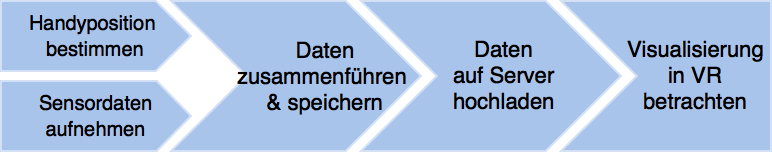
\includegraphics[width=\textwidth]{diagram/dataflow.png}
\end{center}
\end{frame}




\subsection{TrackingManager}

\begin{frame}
\frametitle{Struktur}
\framesubtitle{Tracking Manager}
\begin{itemize}
  	\item	Grobes Tracking durch GPS / Network Provider \pause
 	\item 	Genauere Positionsbestimmung anhand der Signalstärke von markierten Access Points
			\begin{center}
			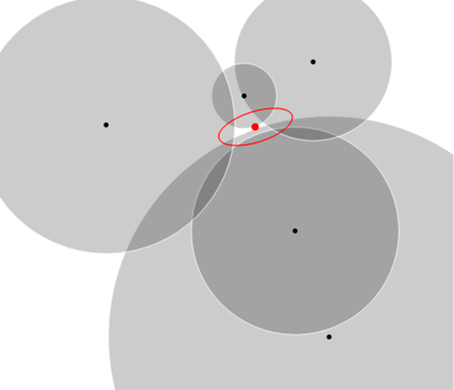
\includegraphics[scale=0.5]{trilateration.png}
			\end{center}
\end{itemize}
\end{frame}

\subsection{WebVR}

\begin{frame}
\frametitle{WebVR}
\only<1,2,4>{
\begin{itemize}
  \item WebVR eine javascript API um VR im browser darzustellen
  \item Einfaches 3d Modell einer Sporthalle \pause
  \item 2 verschiende Visualisierungen
  \begin{itemize}
    \item Daten punkte
    \item<4> Ebene
  \end{itemize}
\end{itemize}}
\only<3>{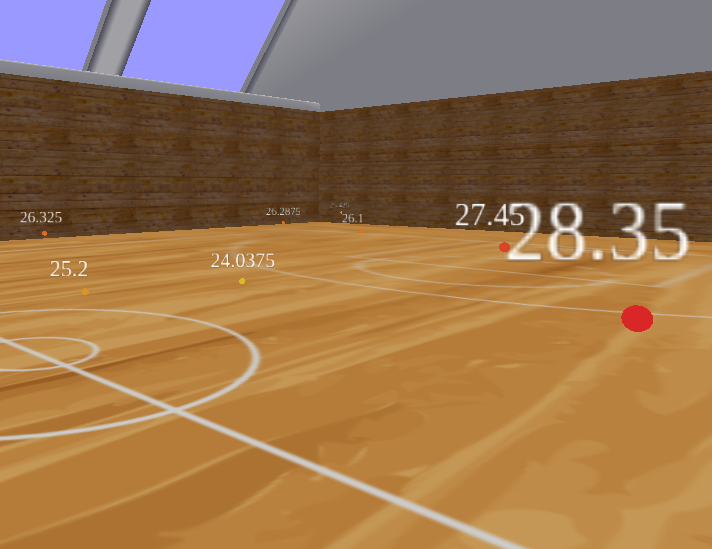
\includegraphics[width=\textwidth]{points.png}}


\end{frame}

\begin{frame}
\frametitle{WebVR}
\begin{itemize}
  \item Interpoliere die Daten
  \item Nutze Inverse Distanzgewichtung's interpolation:
\end{itemize}
\end{frame}

\begin{frame}
\frametitle{WebVR}
  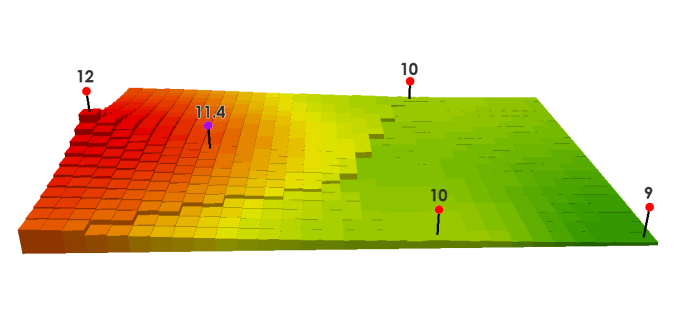
\includegraphics[scale=0.5]{IDW.png}
  \pause
  $$
  u(x) = \frac{\sum_{i=1}^n w_i(x)u_i}{\sum_{i=1}^n w_i(x)}
  $$
\end{frame}


\section{Live-Demonstration}

\begin{frame}
\frametitle{Struktur}
\framesubtitle{Work Flow}
	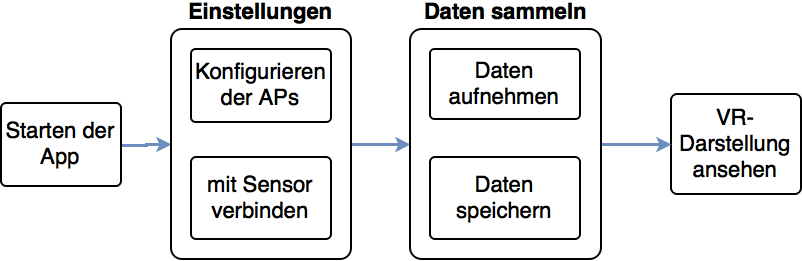
\includegraphics[width=\textwidth]{diagram/workflow.png}
\end{frame}

%Zusatzfolien für eventuelle Erklärungen

\begin{frame}
\frametitle{Bluetooth Manager}
\begin{itemize}
  \item blabla
\end{itemize}
\end{frame}

\begin{frame}
\frametitle{Storage Manager}
\begin{itemize}
  \item blabla
\end{itemize}
\end{frame}

\end{document}
